% mainfile: ../../../../master.tex
\subsection{Connect ART to Bionic}
\label{task:20230102_aosp}

Need to solve the connection between \texttt{libnativehelper\_lazy} and \texttt{art} first.

Change the parameters of \path{WEI_TestFunc} inside \path{libnativehelper_lazy}:
\begin{lstlisting}[language=C++]
// ADDED BY WEI MINN
const void* WEI_TestFunc(){
    typedef const void* (*M)();
    EnsureInitialized();                            
    void* method = g_Methods[k_WEI_TestFunc];           
    return ((M) method)();            
}
\end{lstlisting}

Got this error message when trying to compile:
\begin{lstlisting}
libnativehelper/libnativehelper_lazy.c:287:20: error: array index 16 is past the end of the array (which contains 15 elements) [-Werror,-Warray-bounds]
    void* method = g_Methods[k_WEI_TestFunc];           
                   ^         ~~~~~~~~~~~~~~
\end{lstlisting}

Swap the position of \path{WEI_TestFunc} with \path{k_MethodCount} inside \texttt{MethodIndex} \texttt{enum} of \path{libnativehelper_lazy.c}:
\begin{lstlisting}[language=C++]
// ADDED BY WEI MINN
k_WEI_TestFunc,

// Marker for count of methods
k_MethodCount   
\end{lstlisting}

Android Emulator boot at startup screen and this is message from \texttt{adb logcat}:
\begin{lstlisting}
01-02 13:12:46.793  3799  3799 F zygote  : Failed to find symbol 'WEI_TestFunc' in libnativehelper.so: undefined symbol: WEI_TestFunc
\end{lstlisting}
Because I forgot to put the following implementation inside \texttt{aosp13/libnativehelper/JniInvocation.c}:
\begin{lstlisting}[language=C++]
jint WEI_TestFunc(void* res) {
    ALOG_ALWAYS_FATAL_IF(NULL == g_impl.WEI_TestFunc, "Runtime library not loaded.");
    return g_impl.WEI_TestFunc(res);
}  
\end{lstlisting}

Daemon cannot load \texttt{libnativehelper.so}:
\begin{lstlisting}
01-02 13:22:47.648     0     0 I init    : starting service 'weiminn_daemon'...
01-02 13:22:48.263  1867  1867 D WEIMINN PROJ: STARTING WEIMINN PROJECT
01-02 13:22:50.264  1867  1867 F weiminn_daemon: Failed to load libnativehelper.so: dlopen failed: library "libnativehelper.so" not found
\end{lstlisting}
Tombstone file at \texttt{adb shell cat /data/tombstones/tombstone\_37 > tb.txt}:
\begin{lstlisting}
*** *** *** *** *** *** *** *** *** *** *** *** *** *** *** ***
Build fingerprint: 'Android/sdk_phone_x86_64/emulator_x86_64:13/TD1A.220804.031/eng.weimin.20231119.002237:userdebug/test-keys'
Revision: '0'
ABI: 'x86_64'
Timestamp: 2024-01-02 13:42:01.100413406+0800
Process uptime: 3s
Cmdline: /vendor/bin/hw/weiminn_daemon
pid: 3002, tid: 3002, name: weiminn_daemon  >>> /vendor/bin/hw/weiminn_daemon <<<
uid: 2000
signal 6 (SIGABRT), code -1 (SI_QUEUE), fault addr --------
Abort message: 'Failed to load libnativehelper.so: dlopen failed: library "libnativehelper.so" not found'
    rax 0000000000000000  rbx 0000000000000bba  rcx 00007b83e618d68f  rdx 0000000000000006
    r8  c7632a7a8fbc8b50  r9  c7632a7a8fbc8b50  r10 00007fff3fde6d30  r11 0000000000000217
    r12 00007fff3fde73b8  r13 0000000000000000  r14 00007fff3fde6d28  r15 0000000000000bba
    rdi 0000000000000bba  rsi 0000000000000bba
    rbp 0000000000000001  rsp 00007fff3fde6d20  rip 00007b83e618d68f

backtrace:
        #00 pc 000000000005f68f  /apex/com.android.runtime/lib64/bionic/libc.so (abort+191) (BuildId: 57def992cb1772e13608c8efcafd893b)
        #01 pc 0000000000006a1a  /system/lib64/liblog.so (__android_log_default_aborter+10) (BuildId: acde2d0ef136fd6d1eb2a30987f39d55)
        #02 pc 00000000000075d2  /system/lib64/liblog.so (__android_log_assert+370) (BuildId: acde2d0ef136fd6d1eb2a30987f39d55)
        #03 pc 0000000000001cee  /vendor/bin/hw/weiminn_daemon (InitializeOnce+782) (BuildId: 64dca3fe723864a1e2dd2e698986fb43)
        #04 pc 00000000000ce2c3  /apex/com.android.runtime/lib64/bionic/libc.so (pthread_once+67) (BuildId: 57def992cb1772e13608c8efcafd893b)
        #05 pc 00000000000019c6  /vendor/bin/hw/weiminn_daemon (WEI_TestFunc+22) (BuildId: 64dca3fe723864a1e2dd2e698986fb43)
        #06 pc 0000000000001991  /vendor/bin/hw/weiminn_daemon (main+65) (BuildId: 64dca3fe723864a1e2dd2e698986fb43)
        #07 pc 0000000000050c49  /apex/com.android.runtime/lib64/bionic/libc.so (__libc_init+89) (BuildId: 57def992cb1772e13608c8efcafd893b)

memory near rcx (/apex/com.android.runtime/lib64/bionic/libc.so):
    00007b83e618d660 45e820245c89ffff 4824244489000757  ...\$ .EW...D$$H
    00007b83e618d670 00000000282444c7 8d4cf76349fb6348  .D$(....Hc.Ic.L.
    00007b83e618d680 00000006ba102454 0f050f00000129b8  T$.......)......
    00007b83e618d690 290ffffc2ad20510 100f000000a02484  ...*...).$......
    00007b83e618d6a0 84290ffffc2ab305 b48d480000009024  ..*...).$....H..
    00007b83e618d6b0 0006bf0000009024 075bcfe8d2310000  $.........1...[.
    00007b83e618d6c0 894c00000002bf00 00075bb0e8d231f6  ......L..1...[..
    00007b83e618d6d0 e8c03100000027bf bfc3894800075754  .'...1..TW..H...
    00007b83e618d6e0 45e8c031000000ba 570fc68949000757  ....1..EW..I...W
    00007b83e618d6f0 290f102444290fc0 802484290f202444  ..)D$..)D$ .).$.
    00007b83e618d700 702444290f000000 44290f602444290f  ....)D$p.)D$`.)D
    00007b83e618d710 0f402444290f5024 182444c730244429  $P.)D$@.)D$0.D$.
    00007b83e618d720 20245c89ffffffff 24448900075683e8  .....\$ ..V...D$
    00007b83e618d730 0000282444c74824 f66349fb63480000  $H.D$(....Hc.Ic.
    00007b83e618d740 0006ba1024548d4c 0f00000129b80000  L.T$.......)....
    00007b83e618d750 45e80000007fbf05 cccccccccc00075b  .......E[.......

memory near r10 ([stack]):
    00007fff3fde6d10 0000000000000001 00007b83e618d66b  ........k....{..
    00007fff3fde6d20 c7632a7a8fbc8b50 ffffffffffffffdf  P...z*c.........
    00007fff3fde6d30 0000000000000000 00000000ffffffff  ................
    00007fff3fde6d40 000007d000000bba 0000000000000000  ................
    00007fff3fde6d50 0000000000000000 0000000000000000  ................
    00007fff3fde6d60 0000000000000000 0000000000000000  ................
    00007fff3fde6d70 0000000000000000 0000000000000000  ................
    00007fff3fde6d80 0000000000000000 0000000000000000  ................
    00007fff3fde6d90 0000000000000000 0000000000000000  ................
    00007fff3fde6da0 0000000000000000 0000000000000000  ................
    00007fff3fde6db0 0000000000000000 00007b83e6180998  .............{..
    00007fff3fde6dc0 00007fff3fde6ed0 00007fff3fde73b8  .n.?.....s.?....
    00007fff3fde6dd0 00007fff3fde6ed0 0000000000000000  .n.?............
    00007fff3fde6de0 00007fff3fde73a8 00007b83e67d9a1b  .s.?......}..{..
    00007fff3fde6df0 0000000000000001 00007b83e67da5d3  ..........}..{..
    00007fff3fde6e00 0000003000000020 00007fff3fde72f0   ...0....r.?....

memory near r12 ([stack]):
    00007fff3fde7390 000061461a181010 000061461a17f90e  ....Fa......Fa..
    00007fff3fde73a0 0000000000000001 00007fff3fde827a  ........z..?....
    00007fff3fde73b0 0000000000000000 00007fff3fde8298  ...........?....
    00007fff3fde73c0 00007fff3fde832d 00007fff3fde8340  -..?....@..?....
    00007fff3fde73d0 00007fff3fde8355 00007fff3fde8370  U..?....p..?....
    00007fff3fde73e0 00007fff3fde8383 00007fff3fde839c  ...?.......?....
    00007fff3fde73f0 00007fff3fde83c3 00007fff3fde83ec  ...?.......?....
    00007fff3fde7400 00007fff3fde8419 00007fff3fde8432  ...?....2..?....
    00007fff3fde7410 00007fff3fde844c 00007fff3fde8467  L..?....g..?....
    00007fff3fde7420 00007fff3fde8ace 00007fff3fde8cbb  ...?.......?....
    00007fff3fde7430 00007fff3fde8e74 0000000000000000  t..?............
    00007fff3fde7440 0000000000000021 00007fff3fdef000  !..........?....
    00007fff3fde7450 0000000000000033 00000000000006f0  3...............
    00007fff3fde7460 0000000000000010 00000000178afbfd  ................
    00007fff3fde7470 0000000000000006 0000000000001000  ................
    00007fff3fde7480 0000000000000011 0000000000000064  ........d.......

memory near r14 ([stack]):
    00007fff3fde6d00 00007fff3fde6d28 00007fff3fde73a8  (m.?.....s.?....
    00007fff3fde6d10 0000000000000001 00007b83e618d66b  ........k....{..
    00007fff3fde6d20 c7632a7a8fbc8b50 ffffffffffffffdf  P...z*c.........
    00007fff3fde6d30 0000000000000000 00000000ffffffff  ................
    00007fff3fde6d40 000007d000000bba 0000000000000000  ................
    00007fff3fde6d50 0000000000000000 0000000000000000  ................
    00007fff3fde6d60 0000000000000000 0000000000000000  ................
    00007fff3fde6d70 0000000000000000 0000000000000000  ................
    00007fff3fde6d80 0000000000000000 0000000000000000  ................
    00007fff3fde6d90 0000000000000000 0000000000000000  ................
    00007fff3fde6da0 0000000000000000 0000000000000000  ................
    00007fff3fde6db0 0000000000000000 00007b83e6180998  .............{..
    00007fff3fde6dc0 00007fff3fde6ed0 00007fff3fde73b8  .n.?.....s.?....
    00007fff3fde6dd0 00007fff3fde6ed0 0000000000000000  .n.?............
    00007fff3fde6de0 00007fff3fde73a8 00007b83e67d9a1b  .s.?......}..{..
    00007fff3fde6df0 0000000000000001 00007b83e67da5d3  ..........}..{..

memory near rsp ([stack]):
    00007fff3fde6d00 00007fff3fde6d28 00007fff3fde73a8  (m.?.....s.?....
    00007fff3fde6d10 0000000000000001 00007b83e618d66b  ........k....{..
    00007fff3fde6d20 c7632a7a8fbc8b50 ffffffffffffffdf  P...z*c.........
    00007fff3fde6d30 0000000000000000 00000000ffffffff  ................
    00007fff3fde6d40 000007d000000bba 0000000000000000  ................
    00007fff3fde6d50 0000000000000000 0000000000000000  ................
    00007fff3fde6d60 0000000000000000 0000000000000000  ................
    00007fff3fde6d70 0000000000000000 0000000000000000  ................
    00007fff3fde6d80 0000000000000000 0000000000000000  ................
    00007fff3fde6d90 0000000000000000 0000000000000000  ................
    00007fff3fde6da0 0000000000000000 0000000000000000  ................
    00007fff3fde6db0 0000000000000000 00007b83e6180998  .............{..
    00007fff3fde6dc0 00007fff3fde6ed0 00007fff3fde73b8  .n.?.....s.?....
    00007fff3fde6dd0 00007fff3fde6ed0 0000000000000000  .n.?............
    00007fff3fde6de0 00007fff3fde73a8 00007b83e67d9a1b  .s.?......}..{..
    00007fff3fde6df0 0000000000000001 00007b83e67da5d3  ..........}..{..

memory near rip (/apex/com.android.runtime/lib64/bionic/libc.so):
    00007b83e618d660 45e820245c89ffff 4824244489000757  ...\$ .EW...D$$H
    00007b83e618d670 00000000282444c7 8d4cf76349fb6348  .D$(....Hc.Ic.L.
    00007b83e618d680 00000006ba102454 0f050f00000129b8  T$.......)......
    00007b83e618d690 290ffffc2ad20510 100f000000a02484  ...*...).$......
    00007b83e618d6a0 84290ffffc2ab305 b48d480000009024  ..*...).$....H..
    00007b83e618d6b0 0006bf0000009024 075bcfe8d2310000  $.........1...[.
    00007b83e618d6c0 894c00000002bf00 00075bb0e8d231f6  ......L..1...[..
    00007b83e618d6d0 e8c03100000027bf bfc3894800075754  .'...1..TW..H...
    00007b83e618d6e0 45e8c031000000ba 570fc68949000757  ....1..EW..I...W
    00007b83e618d6f0 290f102444290fc0 802484290f202444  ..)D$..)D$ .).$.
    00007b83e618d700 702444290f000000 44290f602444290f  ....)D$p.)D$`.)D
    00007b83e618d710 0f402444290f5024 182444c730244429  $P.)D$@.)D$0.D$.
    00007b83e618d720 20245c89ffffffff 24448900075683e8  .....\$ ..V...D$
    00007b83e618d730 0000282444c74824 f66349fb63480000  $H.D$(....Hc.Ic.
    00007b83e618d740 0006ba1024548d4c 0f00000129b80000  L.T$.......)....
    00007b83e618d750 45e80000007fbf05 cccccccccc00075b  .......E[.......

memory map (118 entries):
    00006146'1a17e000-00006146'1a17efff r--         0      1000  /vendor/bin/hw/weiminn_daemon (BuildId: 64dca3fe723864a1e2dd2e698986fb43) (load bias 0x1000)
    00006146'1a17f000-00006146'1a17ffff r-x         0      1000  /vendor/bin/hw/weiminn_daemon (BuildId: 64dca3fe723864a1e2dd2e698986fb43) (load bias 0x1000)
    00006146'1a180000-00006146'1a181fff r--         0      2000  /vendor/bin/hw/weiminn_daemon (BuildId: 64dca3fe723864a1e2dd2e698986fb43) (load bias 0x1000)
    00006146'1a182000-00006146'1a182fff rw-      1000      1000  /vendor/bin/hw/weiminn_daemon (BuildId: 64dca3fe723864a1e2dd2e698986fb43) (load bias 0x1000)
    00007b81'53015000-00007b81'83a44fff ---         0  30a30000  [anon:cfi shadow]
    00007b81'83a45000-00007b81'83a45fff r--         0      1000  [anon:cfi shadow]
    00007b81'83a46000-00007b81'90c33fff ---         0   d1ee000  [anon:cfi shadow]
    00007b81'90c34000-00007b81'90c34fff r--         0      1000  [anon:cfi shadow]
    00007b81'90c35000-00007b81'9300dfff ---         0   23d9000  [anon:cfi shadow]
    00007b81'9300e000-00007b81'9300efff r--         0      1000  [anon:cfi shadow]
    00007b81'9300f000-00007b81'd3014fff ---         0  40006000  [anon:cfi shadow]
    00007b81'd3015000-00007b81'd3015fff ---         0      1000
    00007b81'd3016000-00007b81'd3055fff rw-         0     40000  [anon:scudo:primary]
    00007b81'd3056000-00007b81'e3021fff ---         0   ffcc000
    00007b81'e3022000-00007b81'e3061fff rw-         0     40000  [anon:scudo:primary]
    00007b81'e3062000-00007b81'f301bfff ---         0   ffba000
    00007b81'f301c000-00007b81'f305bfff rw-         0     40000  [anon:scudo:primary]
    00007b81'f305c000-00007b82'03019fff ---         0   ffbe000
    00007b82'0301a000-00007b82'03059fff rw-         0     40000  [anon:scudo:primary]
    00007b82'0305a000-00007b83'e3014fff ---         0  1dffbb000
    00007b83'e3015000-00007b83'e3063fff r--         0     4f000  /apex/com.android.vndk.v33/lib64/libc++.so (BuildId: fa40b55330a4a2a3eca001f4cae01033) (load bias 0x1000)
    00007b83'e3064000-00007b83'e30c1fff r-x     4e000     5e000  /apex/com.android.vndk.v33/lib64/libc++.so (BuildId: fa40b55330a4a2a3eca001f4cae01033) (load bias 0x1000)
    00007b83'e30c2000-00007b83'e30c8fff r--     ab000      7000  /apex/com.android.vndk.v33/lib64/libc++.so (BuildId: fa40b55330a4a2a3eca001f4cae01033) (load bias 0x1000)
    00007b83'e30c9000-00007b83'e30c9fff rw-     b1000      1000  /apex/com.android.vndk.v33/lib64/libc++.so (BuildId: fa40b55330a4a2a3eca001f4cae01033) (load bias 0x1000)
    00007b83'e30ca000-00007b83'e30ccfff rw-         0      3000  [anon:.bss]
    00007b83'e31cf000-00007b83'e31d1fff r--         0      3000  /system/lib64/libnetd_client.so (BuildId: 0ba64f6d28b890efbf31d3d283147280) (load bias 0x1000)
    00007b83'e31d2000-00007b83'e31d2fff ---         0      1000
    00007b83'e31d3000-00007b83'e31d6fff r-x      3000      4000  /system/lib64/libnetd_client.so (BuildId: 0ba64f6d28b890efbf31d3d283147280) (load bias 0x1000)
    00007b83'e31d7000-00007b83'e31d7fff r--      6000      1000  /system/lib64/libnetd_client.so (BuildId: 0ba64f6d28b890efbf31d3d283147280) (load bias 0x1000)
    00007b83'e31d8000-00007b83'e31d8fff rw-      6000      1000  /system/lib64/libnetd_client.so (BuildId: 0ba64f6d28b890efbf31d3d283147280) (load bias 0x1000)
    00007b83'e3200000-00007b83'e5ffffff ---         0   2e00000
    00007b83'e6057000-00007b83'e6057fff r--         0      1000  /apex/com.android.runtime/lib64/bionic/libdl.so (BuildId: efd82935135bb07f6cf82127470e5900) (load bias 0x1000)
    00007b83'e6058000-00007b83'e6058fff r-x         0      1000  /apex/com.android.runtime/lib64/bionic/libdl.so (BuildId: efd82935135bb07f6cf82127470e5900) (load bias 0x1000)
    00007b83'e6059000-00007b83'e6059fff r--         0      1000  /apex/com.android.runtime/lib64/bionic/libdl.so (BuildId: efd82935135bb07f6cf82127470e5900) (load bias 0x1000)
    00007b83'e605a000-00007b83'e605afff ---         0      1000
    00007b83'e605b000-00007b83'e605bfff r--         0      1000  [anon:.bss]
    00007b83'e6096000-00007b83'e60b4fff r--         0     1f000  /apex/com.android.runtime/lib64/bionic/libm.so (BuildId: 9cfa4f2cea749f828172a4bab94dcf95) (load bias 0x1000)
    00007b83'e60b5000-00007b83'e60e5fff r-x     1e000     31000  /apex/com.android.runtime/lib64/bionic/libm.so (BuildId: 9cfa4f2cea749f828172a4bab94dcf95) (load bias 0x1000)
    00007b83'e60e6000-00007b83'e60e6fff r--     4e000      1000  /apex/com.android.runtime/lib64/bionic/libm.so (BuildId: 9cfa4f2cea749f828172a4bab94dcf95) (load bias 0x1000)
    00007b83'e60e7000-00007b83'e60e7fff rw-     4e000      1000  /apex/com.android.runtime/lib64/bionic/libm.so (BuildId: 9cfa4f2cea749f828172a4bab94dcf95) (load bias 0x1000)
    00007b83'e612e000-00007b83'e6171fff r--         0     44000  /apex/com.android.runtime/lib64/bionic/libc.so (BuildId: 57def992cb1772e13608c8efcafd893b) (load bias 0x1000)
    00007b83'e6172000-00007b83'e6204fff r-x     43000     93000  /apex/com.android.runtime/lib64/bionic/libc.so (BuildId: 57def992cb1772e13608c8efcafd893b) (load bias 0x1000)
    00007b83'e6205000-00007b83'e6209fff r--     d5000      5000  /apex/com.android.runtime/lib64/bionic/libc.so (BuildId: 57def992cb1772e13608c8efcafd893b) (load bias 0x1000)
    00007b83'e620a000-00007b83'e620afff rw-     d9000      1000  /apex/com.android.runtime/lib64/bionic/libc.so (BuildId: 57def992cb1772e13608c8efcafd893b) (load bias 0x1000)
    00007b83'e620b000-00007b83'e675cfff rw-         0    552000  [anon:.bss]
    00007b83'e675d000-00007b83'e675dfff r--         0      1000  [anon:.bss]
    00007b83'e675e000-00007b83'e6765fff rw-         0      8000  [anon:.bss]
    00007b83'e676f000-00007b83'e67d2fff rw-         0     64000  [anon:linker_alloc]
    00007b83'e67d3000-00007b83'e67d7fff r--         0      5000  /system/lib64/liblog.so (BuildId: acde2d0ef136fd6d1eb2a30987f39d55) (load bias 0x1000)
    00007b83'e67d8000-00007b83'e67e1fff r-x      4000      a000  /system/lib64/liblog.so (BuildId: acde2d0ef136fd6d1eb2a30987f39d55) (load bias 0x1000)
    00007b83'e67e2000-00007b83'e67e2fff r--      d000      1000  /system/lib64/liblog.so (BuildId: acde2d0ef136fd6d1eb2a30987f39d55) (load bias 0x1000)
    00007b83'e67e3000-00007b83'e67e3fff rw-      d000      1000  /system/lib64/liblog.so (BuildId: acde2d0ef136fd6d1eb2a30987f39d55) (load bias 0x1000)
    00007b83'e6800000-00007b83'e95fffff ---         0   2e00000
    00007b83'e9621000-00007b83'e9640fff r--         0     20000  /dev/__properties__/u:object_r:heapprofd_prop:s0
    00007b83'e9641000-00007b83'e9660fff r--         0     20000  /dev/__properties__/u:object_r:libc_debug_prop:s0
    00007b83'e9661000-00007b83'e9669fff r--         0      9000  /apex/com.android.vndk.v33/lib64/libcutils.so (BuildId: 43606b529d94720adf378693c75eca35) (load bias 0x1000)
    00007b83'e966a000-00007b83'e9675fff r-x      8000      c000  /apex/com.android.vndk.v33/lib64/libcutils.so (BuildId: 43606b529d94720adf378693c75eca35) (load bias 0x1000)
    00007b83'e9676000-00007b83'e9677fff r--     13000      2000  /apex/com.android.vndk.v33/lib64/libcutils.so (BuildId: 43606b529d94720adf378693c75eca35) (load bias 0x1000)
    00007b83'e9678000-00007b83'e9678fff rw-     14000      1000  /apex/com.android.vndk.v33/lib64/libcutils.so (BuildId: 43606b529d94720adf378693c75eca35) (load bias 0x1000)
    00007b83'e9683000-00007b83'e9696fff r--         0     14000  /apex/com.android.vndk.v33/lib64/libbase.so (BuildId: 314908d7976b6d0a21139dcdb1a359d4) (load bias 0x1000)
    00007b83'e9697000-00007b83'e96c2fff r-x     13000     2c000  /apex/com.android.vndk.v33/lib64/libbase.so (BuildId: 314908d7976b6d0a21139dcdb1a359d4) (load bias 0x1000)
    00007b83'e96c3000-00007b83'e96c3fff r--     3e000      1000  /apex/com.android.vndk.v33/lib64/libbase.so (BuildId: 314908d7976b6d0a21139dcdb1a359d4) (load bias 0x1000)
    00007b83'e96c4000-00007b83'e96c4fff rw-     3e000      1000  /apex/com.android.vndk.v33/lib64/libbase.so (BuildId: 314908d7976b6d0a21139dcdb1a359d4) (load bias 0x1000)
    00007b83'e96c5000-00007b83'e96c5fff rw-         0      1000  [anon:.bss]
    00007b83'e96e4000-00007b83'e9703fff r--         0     20000  /dev/__properties__/u:object_r:gwp_asan_prop:s0
    00007b83'e9704000-00007b83'e9752fff r--         0     4f000  /system/lib64/libc++.so (BuildId: 7de31e7c740e102016d16ce256f97d3a) (load bias 0x1000)
    00007b83'e9753000-00007b83'e97b0fff r-x     4e000     5e000  /system/lib64/libc++.so (BuildId: 7de31e7c740e102016d16ce256f97d3a) (load bias 0x1000)
    00007b83'e97b1000-00007b83'e97b7fff r--     ab000      7000  /system/lib64/libc++.so (BuildId: 7de31e7c740e102016d16ce256f97d3a) (load bias 0x1000)
    00007b83'e97b8000-00007b83'e97b8fff rw-     b1000      1000  /system/lib64/libc++.so (BuildId: 7de31e7c740e102016d16ce256f97d3a) (load bias 0x1000)
    00007b83'e97b9000-00007b83'e97bbfff rw-         0      3000  [anon:.bss]
    00007b83'e97c1000-00007b83'e97e0fff r--         0     20000  /dev/__properties__/u:object_r:debug_prop:s0
    00007b83'e97e1000-00007b83'e9800fff r--         0     20000  /dev/__properties__/properties_serial
    00007b83'e9801000-00007b83'e9801fff rw-         0      1000  [anon:bionic_alloc_small_objects]
    00007b83'e981c000-00007b83'e982dfff r--         0     12000  /dev/__properties__/property_info
    00007b83'e9832000-00007b83'e9851fff r--         0     20000  /dev/__properties__/u:object_r:build_prop:s0
    00007b83'e9852000-00007b83'e9871fff r--         0     20000  /dev/__properties__/u:object_r:log_tag_prop:s0
    00007b83'e9872000-00007b83'e9891fff r--         0     20000  /dev/__properties__/u:object_r:vendor_socket_hook_prop:s0
    00007b83'e9892000-00007b83'e9959fff r--         0     c8000  [anon:linker_alloc]
    00007b83'e995a000-00007b83'e9979fff r--         0     20000  /dev/__properties__/u:object_r:vndk_prop:s0
    00007b83'e997b000-00007b83'e9982fff rw-         0      8000  [anon:bionic_alloc_small_objects]
    00007b83'e9983000-00007b83'e9983fff rw-         0      1000  [anon:bionic_alloc_lob]
    00007b83'e9984000-00007b83'e9985fff rw-         0      2000  [anon:bionic_alloc_small_objects]
    00007b83'e9986000-00007b83'e9988fff rw-         0      3000  [anon:System property context nodes]
    00007b83'e9989000-00007b83'e9989fff ---         0      1000
    00007b83'e998a000-00007b83'e998cfff rw-         0      3000  [anon:stack_and_tls:main]
    00007b83'e998d000-00007b83'e998dfff ---         0      1000
    00007b83'e998e000-00007b83'e998ffff rw-         0      2000  [anon:bionic_alloc_lob]
    00007b83'e9992000-00007b83'e9996fff rw-         0      5000  [anon:bionic_alloc_small_objects]
    00007b83'e9997000-00007b83'e99fafff r--         0     64000  [anon:linker_alloc]
    00007b83'e99fb000-00007b83'e99fbfff rw-         0      1000  [anon:bionic_alloc_small_objects]
    00007b83'e99fc000-00007b83'e9a1bfff r--         0     20000  /dev/__properties__/u:object_r:debug_prop:s0
    00007b83'e9a1c000-00007b83'e9a3bfff r--         0     20000  /dev/__properties__/u:object_r:build_prop:s0
    00007b83'e9a3c000-00007b83'e9a3cfff ---         0      1000
    00007b83'e9a3d000-00007b83'e9a44fff rw-         0      8000
    00007b83'e9a45000-00007b83'e9a45fff ---         0      1000
    00007b83'e9a46000-00007b83'e9a65fff r--         0     20000  /dev/__properties__/properties_serial
    00007b83'e9a66000-00007b83'e9a68fff rw-         0      3000  [anon:System property context nodes]
    00007b83'e9a69000-00007b83'e9a7afff r--         0     12000  /dev/__properties__/property_info
    00007b83'e9a7b000-00007b83'e9adefff r--         0     64000  [anon:linker_alloc]
    00007b83'e9adf000-00007b83'e9ae0fff rw-         0      2000  [anon:bionic_alloc_small_objects]
    00007b83'e9ae1000-00007b83'e9ae1fff r--         0      1000  [anon:atexit handlers]
    00007b83'e9ae2000-00007b83'e9ae2fff ---         0      1000
    00007b83'e9ae3000-00007b83'e9aeafff rw-         0      8000  [anon:thread signal stack]
    00007b83'e9aeb000-00007b83'e9aebfff rw-         0      1000  [anon:arc4random data]
    00007b83'e9aec000-00007b83'e9aecfff rw-         0      1000  [anon:abort message]
    00007b83'e9aed000-00007b83'e9aedfff r--         0      1000  [anon:atexit handlers]
    00007b83'e9aee000-00007b83'e9aeefff rw-         0      1000  [anon:arc4random data]
    00007b83'e9aef000-00007b83'e9b32fff r--         0     44000  /apex/com.android.runtime/bin/linker64 (BuildId: 88b9a0b1efb561bd3d51b1972ee9b024) (load bias 0x1000)
    00007b83'e9b33000-00007b83'e9c27fff r-x     43000     f5000  /apex/com.android.runtime/bin/linker64 (BuildId: 88b9a0b1efb561bd3d51b1972ee9b024) (load bias 0x1000)
    00007b83'e9c28000-00007b83'e9c2ffff r--    137000      8000  /apex/com.android.runtime/bin/linker64 (BuildId: 88b9a0b1efb561bd3d51b1972ee9b024) (load bias 0x1000)
    00007b83'e9c30000-00007b83'e9c31fff rw-    13e000      2000  /apex/com.android.runtime/bin/linker64 (BuildId: 88b9a0b1efb561bd3d51b1972ee9b024) (load bias 0x1000)
    00007b83'e9c32000-00007b83'e9c3afff rw-         0      9000  [anon:.bss]
    00007b83'e9c3b000-00007b83'e9c3bfff r--         0      1000  [anon:.bss]
    00007b83'e9c3c000-00007b83'e9c3dfff rw-         0      2000  [anon:.bss]
    00007fff'3fdc8000-00007fff'3fde8fff rw-         0     21000  [stack]
    00007fff'3fdeb000-00007fff'3fdeefff r--         0      4000  [vvar]
    00007fff'3fdef000-00007fff'3fdeffff r-x         0      1000  [vdso]
    ffffffff'ff600000-ffffffff'ff600fff --x         0      1000  [vsyscall]
--------- tail end of log main
01-02 13:41:59.096  3002  3002 D WEIMINN PROJ: STARTING WEIMINN PROJECT
01-02 13:42:01.096  3002  3002 F weiminn_daemon: Failed to load libnativehelper.so: dlopen failed: library "libnativehelper.so" not found

open files:
    fd 0: /dev/null (unowned)
    fd 1: /dev/null (unowned)
    fd 2: /dev/null (unowned)
    fd 3: socket:[57035] (unowned)
    fd 4: /dev/pmsg0 (unowned)
--------- log main
01-02 13:41:59.096  3002  3002 D WEIMINN PROJ: STARTING WEIMINN PROJECT
01-02 13:42:01.096  3002  3002 F weiminn_daemon: Failed to load libnativehelper.so: dlopen failed: library "libnativehelper.so" not found    
\end{lstlisting}
I think it's because we are calling into \texttt{libnativehelper.so} without loading it first using \texttt{JniInvocation}. So we need to figure out the way to initialize JNI inovation and store the instance.

Test out calling just \texttt{libnativehelper.c} instead of all the way into \texttt{art} modules.

% \subsubsection{Configure SELinux}

% Change the \texttt{seclabel} of the service inside \path{AOSP/device/generic/goldfish/app/init.weiminn.rc} to:
% \begin{lstlisting}
% seclabel u:r:shell:s0
% \end{lstlisting}
% from
% \begin{lstlisting}
% seclabel u:r:weiminn_daemon:s0
% \end{lstlisting}
% and the error message changed to 
% \begin{lstlisting}
% [61133.720482] init: starting service 'weiminn_daemon'...
% [61133.721480] init: cannot setexeccon('u:r:weiminn_daemon:s0') for weiminn_daemon: Invalid argument
% [61133.722452] init: Service 'weiminn_daemon' (pid 14423) exited with status 6
% [61133.722745] init: Sending signal 9 to service 'weiminn_daemon' (pid 14423) process group...
% [61133.723107] libprocessgroup: Successfully killed process cgroup uid 0 pid 14423 in 0ms    
% \end{lstlisting}
% in \texttt{dmesg}, and 
% \begin{lstlisting}
% 12-25 10:57:23.010     0     0 I init    : starting service 'weiminn_daemon'...
% 12-25 10:57:23.011     0     0 F init    : cannot setexeccon('u:r:weiminn_daemon:s0') for weiminn_daemon: Invalid argument
% 12-25 10:57:23.011     0     0 I init    : Service 'weiminn_daemon' (pid 14441) exited with status 6
% 12-25 10:57:23.012     0     0 I init    : Sending signal 9 to service 'weiminn_daemon' (pid 14441) process group...
% 12-25 10:57:23.012     0     0 I libprocessgroup: Successfully killed process cgroup uid 0 pid 14441 in 0ms
% \end{lstlisting}
% inside \texttt{adb logcat}.

% The error seems to be come from the SELinux type \texttt{weiminn\_daemon} inside the \texttt{init.rc}. So, I'm gonna change back to \texttt{seclabel u:r:shell:s0}, and inspect the \texttt{avc: denied} message, which tells us that the process is \texttt{init} type, and the binary is \texttt{vendor\_file} type.

% Add Access Vector rule to allow execute on \texttt{vendor\_file} type. Alternatively, I put \texttt{setenforce 0} inside \texttt{adb shell}, and voila!

% Log to \texttt{logcat} every time ART executes a Java method\footnote{\url{https://stackoverflow.com/questions/33478647/android-app-java-jni-call-hooking-strategies}, \url{https://www.youtube.com/watch?v=mFq0vNvUgj8}}. But it requires to be NOT on emulator, so scrap that plan.

% The security context, together with the run-time user that the process is in, would define what the process is allowed to do.

% \begin{lstlisting}[language=sh]
% ps -ef # -e gives all processes, -f gives more info, -Z gives security context

% ls -ld dir # shows the permissions related to this directory
% ls -ldZ dir # shows the permissions and also SELinux context
% \end{lstlisting}

% \begin{itemize}
% \item \textbf{Domain.} The context of the process that is acting upon something.
% \item \textbf{Type.} The context of the resource on which the process is acting.
% \item \textbf{Class.} The object class of the resource (e.g. \textit{file} or \textit{socket}).
% \item \textbf{Permissions.} The permissions that are allowed given the \textit{domain}, \textit{type} and \textit{class}.
% \end{itemize}

% SELinux rule syntax:
% \begin{lstlisting}
% allow <domain> <type>:<class> { <permissions> };
% \end{lstlisting}

% \subsubsection{Decoding Permission Denial Message}

% Message:
% \begin{lstlisting}
% type=AVC msg=audit(1363289005.532:184): avc:  denied  { read } for  pid=29199 comm="Trace" 
% name="online" dev="sysfs" ino=30 scontext=staff_u:staff_r:googletalk_plugin_t 
% tcontext=system_u:object_r:sysfs_t tclass=file
% \end{lstlisting}

% \begin{longtable}{p{.15\linewidth}p{.15\linewidth}p{.65\linewidth}} 
% \toprule
% Log part & Name & Description \\
% \midrule
% \endhead

% \texttt{type=AVC}
% &Log type
% &Only in the \texttt{audit.log} file; it informs the user what kind of audit log type this is. 
% \\

% \texttt{msg=audit(1363289005.532:184)}
% &Timestamp
% &Timestamp in seconds since epoch, meaning the number of seconds since January 1st, 1970. You can convert this to a more human readable format using date -d @ followed by the number, like so: \texttt{date -d @1363292159.532}.
% \\

% \texttt{avc:}
% &Log type (again)
% &
% \\

% \texttt{denied}
% &State (if enforced)
% &What SELinux did, which can be either \texttt{denied} or \texttt{granted}. Note that, if SELinux is in premissive mode, then it will still log as \texttt{denied} even though it was enforced.
% \\

% \texttt{\{ read \}}
% &Permission
% &Ther permission that was requested or executed. In this case, it is a read operation. Sometimes the permission contains a set like \texttt{\{ read write \}} but in most cases, it is a single permission request.
% \\

% \texttt{for pid=29199}
% &Process PID
% &Ther process identifier of the process that took the action.
% \\

% \texttt{comm="Trace"}
% &Process CMD
% &The process command (without arguments, and limited to 15 characters), which helps users identify what the process was in case the process is already gone (a PID is only useful if the process is still running)
% \\

% \texttt{name="online"}
% &Target name
% &The name of the target (in this case, file name). This field depends heavily on the target itself; it can also be \texttt{path=}, \texttt{capability=}, \texttt{src=} and more. But in those cases, its purposes should be clear from the rest of the log.
% \\

% \texttt{dev="sysfs"}
% &Device
% &Device on which the target (in case of a file or file system). In this case, the device is \texttt{sysfs} so we have the hint immediately that this is for something inside \texttt{/sys}. Other valid example are \texttt{dev=md-0}, \texttt{dev=sda1}, or \texttt{dev=tmpfs}.
% \\

% \texttt{ino=30}
% &inode number
% &The inode number of the target file. In this case, since we know it is on the \texttt{sysfs} file system, we can look for this file using: \texttt{find /sys -xdev -inum 30}
% \\

% \texttt{scontent=staff\_u:staff\_r:googletalk\_plugin\_t}
% &Source context
% &The security context of the process (the domain)
% \\

% \texttt{tcontext=system\_u:object\_r:sysfs\_t}
% &Target context
% &The security context of the target resource (in this case the file)
% \\

% \texttt{tclass=file}
% &Target class
% &The class of the target.
% \\

% \midrule
% \caption{Permission Denied Syntax} 
% \label{tab:permissiondeniedsyntax}
% \end{longtable}


% \subsubsection{SELinux Architecture}

% SELinux consists of four main components: object managers (OM), access vector cache (AVC), security server, and security policy as show below:
% \begin{figure}[H]
%     \centering
%     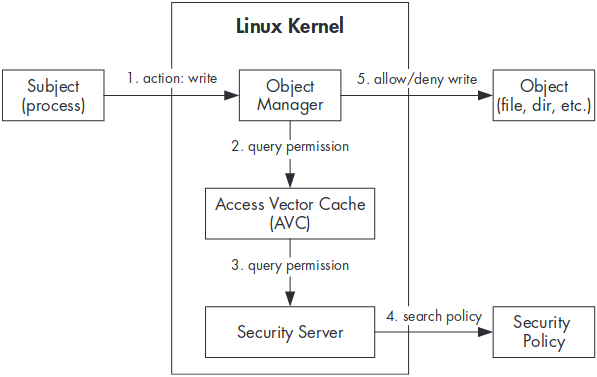
\includegraphics[width=.85\linewidth]{entries/2023/12/10/selinux.png}
%     \caption{SELinux Components}
%     \label{fig:selinux}
% \end{figure}
% When a subject asks to perform an action on an SELinux object, the associated object manager queries the AVC to see if the attempted action is allowed. If the AVC contains a cached security decision for the request, the AVC returns it to the OM which enforces the decision by allowing or denying the action. If the cache does not contain a matching security decision based on the currently loaded policy and returns it to the AVC, which caches it. The AVC in turn returns it to the OM which ultimately enforces the decision. The security server is part of the kernel, while the policy is loaded from userspace via a series of functions contained in the supporting userspace library.

% \subsubsection{SELinux Modes}

% SELinux has 3 modes:
% \begin{itemize}
% \item \textbf{Disabled.} No policy is loaded and only the default DAC security is enforced.
% \item \textbf{Permissive.} The policy is loaded and object access is checked, but access denial is only logged - not enforced.
% \item \textbf{Enforcing.} The security policy is both loaded and enforced, with violations logged.
% \end{itemize}

% SELinux mode can be checked and changed with the \texttt{getenforce} and \texttt{setenforce} commands:
% \begin{lstlisting}[language=sh]
% # getenforce
% Enforcing
% # setenforce 0
% # getenforce
% Permissive
% \end{lstlisting}
% The mode set with \texttt{setenforce} is not persistent and will be reset to the default mode when the device reboots.

% \subsubsection{Mandatory Access Control}

% \begin{itemize}
% \item \textbf{Subjects} are usually running processes that perform actions on objects,
% \item \textbf{Objects} are OS-level resources managed by the kernel (processes can also be objects), and
% \item \textbf{Actions} are carried out only if the security policy allows it.
% \end{itemize}
% Both subjects and objects have a set of security attributes (collectively known as the security context) which the OS queries in order to decide whether the requested action should be allowed or not. When SELinux is enabled, subjects cannot bypass or influence policy rules; therefore, the policy is mandatory. The MAC policy is only consulted if the DAC allows access to the resource. If the DAC denies access, the denial is taken as the final security decision. 

% % \noindent
% SELinux support two forms of MAC: \textit{type enforcement (TE)} and \textit{multi-level security (MLS)}. 
% MLS is used to enforce different levels of access to restricted information and is not used in Android. 
% TE implemented in SELinux requires that all subjects and objects have an associated type and SELinux uses this type to enforce the rules of its security policy. A \textit{type} is simply a string that's defined in the policy and assoicated with objects or subjects. Subject types references processes or groups of processes and are also referred to as \textit{domains}. Types referring to objects usually specify the role an object plays within a policy, such as system file, application data file, and so on. The type (or domain) is an integral part of the security context.

% \subsubsection{Security Contexts}

% A \textit{security context} (also referred to as a \textit{security label}, or just \textit{label}) is a string with four fields delimited with colons: username, role, type, and an optional MLS security range. 

% An SELinux username is typically asosciated with a group of class of users; for example \path{user_u} for unprivileged users and \path{admin_u} for administrators. Users can be associated with one or more domain type. The type is used to group processes in a domain or to specify an object logical type. In Android context, the user is fixed to \texttt{u}.

% The security range (or level) is used to implement ML and specifies the security levels a subject is allowed to access. In Android context, the security range is fixed to \texttt{s0}.

% By specifying the option \texttt{-Z}, we can see the security context of the processes running:
% \begin{lstlisting}[language=sh]
% # ps -Z
% u:r:su:s0   root    1847    1834    10842820    3384    sigsuspe+
% u:r:su:s0   root    1878    1847    10800932    3572    0  
% \end{lstlisting}
% Subjects inherit the security context of their parent process, or they can change their context via \textit{domain transition} which can be made automatic. For example, all system daemons are started by the \textit{init} process, which has \textit{u:r:init:s0} secuirty context, they would normally inherit this context, but Android's SELinux poly uses automatic domain transitions to set a dedicated domain to each daemon as need.

% Similarly the context of files can be revealed using the \texttt{-Z} option:
% \begin{lstlisting}[language=sh]
% # ls -Z
% lrwxr-xr-x 1 root shell u:object_r:system_file:s0                         6 2023-11-19 00:50 uuidgen -> toybox
% -rwxr-xr-x 1 root shell u:object_r:vdc_exec:s0                       101920 2023-11-19 00:50 vdc
% -rwxr-xr-x 1 root shell u:object_r:viewcompiler_exec:s0              277472 2023-11-19 00:50 viewcompiler
% lrwxr-xr-x 1 root shell u:object_r:system_file:s0                         6 2023-11-19 00:50 vmstat -> toybox
% -rwxr-xr-x 1 root shell u:object_r:vold_exec:s0                      994368 2023-11-19 00:50 vold
% -rwxr-xr-x 1 root shell u:object_r:vold_prepare_subdirs_exec:s0       38576 2023-11-19 00:50 vold_prepare_subdirs
% -rwxr-xr-x 1 root shell u:object_r:system_file:s0                       169 2023-11-19 01:02 vr
% lrwxr-xr-x 1 root shell u:object_r:system_file:s0                         6 2023-11-19 00:50 watch -> toybox
% -rwxr-xr-x 1 root shell u:object_r:watchdogd_exec:s0                  10760 2023-11-19 00:50 watchdogd
% lrwxr-xr-x 1 root shell u:object_r:system_file:s0                         6 2023-11-19 00:50 wc -> toybox
% lrwxr-xr-x 1 root shell u:object_r:system_file:s0                         6 2023-11-19 00:50 which -> toybox
% lrwxr-xr-x 1 root shell u:object_r:system_file:s0                         6 2023-11-19 00:50 whoami -> toybox
% -rwxr-xr-x 1 root shell u:object_r:wificond_exec:s0                  393248 2023-11-19 00:50 wificond

% \end{lstlisting}
% For objects, the security context is persistent and is usually stored as an extended attribute in the file's metadata. Objects typically inherit the type label of their parent (their directory), and can change to a different label via \textit{type transition}.

% \subsubsection{Security Policy}

% Security policies are used by the security server in the kernel to allow or disallow access to kernel objects at runtime. For performance reasons, the policy is typically in binary form generated by compiling a number of policy source files. \textit{Statements} define policy entities such as types, users, and roles. \textit{Rules} allow or deny access to objects (access vector rules); and designate how default users, roles, and types are assigned (default rules). \footnote{Type, attribute and permission statements make up the bulk of a security policy.}

% The listing below declares \path{file_type} and \texttt{domain} attributes, declares \path{system_data_file} type and associates it with \path{file_type} and \path{data_file_type} attributes, declares \path{untrusted_app} type and associate it with \texttt{domain} attribute:
% \begin{lstlisting}
% attribute file_type;
% attribute domain;

% type system_data_file, file_type, data_file_type;
% type untrusted_app, domain;
% \end{lstlisting}

% \texttt{user} statement declares an SELinux user identifier, associates it with its role(s), and optionally specifies its default security level and the range of security levels that user can access:
% \begin{lstlisting}
% user u roles { r } level s0 range s0 - mls_systemhigh;
% \end{lstlisting}
% The \textit{u} user is associated with the \textit{r} role (inside the braces), which in turn is declared using the \texttt{role} statement as show below:
% \begin{lstlisting}
% role r;
% role r types domain;
% \end{lstlisting}
% The second statement associates the \textit{r} role with the \texttt{domain} attribute, which marks it as a role assigned to processes (domains).

% \texttt{permissive} statement allows a named domain to run in permissive mode\footnote{Most domains in Android's current base policy are permissive.}:
% \begin{lstlisting}
% type adbd, domain;
% permissive adbd;
% --snip--
% \end{lstlisting}

% The \texttt{class} statement defines an SELinux object class. Object classes and their associated permissions are determined by the respected object manager implementations in Linux kernel, and are static within a policy. Object classes are usually defined in the \textit{security\_classes} policy source file:
% \begin{lstlisting}
% --snip-
% # file-related classes 
% class filesystem 
% class file 
% class dir 
% class fd 
% class lnk_file 
% class chr_file 
% class blk_file 
% class sock_file 
% class fifo_file 
% --snip--
% \end{lstlisting}

% Access vectors are usually defined and associated with object classes in a policy source file called \textit{access\_vectors}. Permissions can be either class-specific or inheritable by one or more object classes, in which case they're defined with the \texttt{common} keyword. Below is the definition of the set of permissions common to all file objects, and the association of the \texttt{dir} class (which represents directories), and a set of directory-specific permissions (\textit{add\_name}, \textit{remove\_name}, and so on):
% \begin{lstlisting}
% --snip--
% common file 
% { 
%     ioctl 
%     read
%     write 
%     create 
%     getattr 
%     setattr 
%     lock 
%     --snip--
% } 
% --snip--
% class dir 
% inherits file 
% { 
%     add_name 
%     remove_name 
%     reparent 
%     search 
%     rmdir 
%     --snip--
% }
% --snip--
% \end{lstlisting}

% \subsubsection{Type Transition Rules}

% Type enforcement rules and access vector rules typically make the bulk of an SELinux policy. The most commonly used type of enforcement rule is the \path{type_transition} rule, which specifies when domain and type transitions are allowed:
% \begin{lstlisting}
% # from wpa_supplicant.te

% # wpa - wpa supplicant or equivalent 
% type wpa, domain; 
% permissive wpa;
% type wpa_exec, exec_type, file_type; 

% init_daemon_domain(wpa)
% unconfined_domain(wpa)

% # wpa_supplicant daemon uses the type transition rule to associate the control sockets it creates in /data/misc/wifi directory with wpa_socket type
% type_transition wpa             wifi_data_file: sock_file   wpa_socket;
% #               source type     target type     class       type of object after the transition
% \end{lstlisting}

% \subsubsection{Domain Transition Rules}

% Most daemons are associated with a dedicated and use domain transitions to switch their domain when started. This is typically accomplished using the \path{init_daemon_domain()} macro, which under the hood is implemented using the \path{type_transition} keyword. The \path{init_daemon_domain()} macro takes one parameter and is defined in the \textit{te\_macros} file using two other macros: \path{domain_trans()} and \path{domain_auto_trans()} which are used to allow transition to a new domain and to execute the transition automatically, respectively:
% \begin{lstlisting}
% # Domain transition macros definition int the te_macros file

% # domain_trans(olddomain, type, newdomain) 
% define(`domain_trans', ` 
% allow $1 $2:file { getattr open read execute }; 
% allow $1 $3:process transition; 
% allow $3 $2:file { entrypoint read execute }; 
% allow $3 $1:process sigchld; 
% dontaudit $1 $3:process noatsecure; 
% allow $1 $3:process { siginh rlimitinh }; ')
% # domain_auto_trans(olddomain, type, newdomain) 
% define(`domain_auto_trans', ` 
% domain_trans($1,$2,$3) 
% type_transition $1 $2:process $3; ')
% # init_daemon_domain(domain) 
% define(`init_daemon_domain', ` 
% domain_auto_trans(init, $1_exec, $1) 
% tmpfs_domain($1) ') 
% --snip--
% \end{lstlisting}
% The lines beginning with the \texttt{allow} keyword are access vector (AV) rules.

% \subsubsection{Access Vector Rules}

% AV rules define what privileges processes have at runtime by specifying the set of permissions they have over their target objects:
% \begin{lstlisting}
% # Format of AV rules
% rule_name source_type target_type : class perm_set;
% \end{lstlisting}

% The \path{rule_name} can be \texttt{allow}, \texttt{dontallow}, \texttt{auditallow}, \texttt{neverallow}. 
% \texttt{allow} specifies the operations that a subject (process) of the specified source type is allowed to perform on an object of the target type and class specified in the rule.
% \texttt{auditallow} rule is used with \texttt{allow} to record audit events when an operation is allowed.
% \texttt{dontaudit} rule is used to suppress the auditing of denial messages when a specified event is known to be safe.
% \texttt{neverallow} rule says that the declared operation should never be allowed even if an explicit \texttt{allow} rule that allows it exists.

% To form a rule, \path{source_type} and \path{target_type} elements are replaced with one or more previously defined \texttt{type} or \texttt{attribute} identifiers, where \path{source_type} is the identifier of a subject (process), and \path{target_type} is the identifer of an object the process is trying to access. The \texttt{class} element is replaced with the object class of the target, and \path{perm_set} specifies the set of permissions that the source process has over the target object. You can specify multiple types, classes, and permissions by enclosing them in braces (\path{{}}). In addition, so rules support use of the wildcard (\path{*}) and complement(\path{~}) operators, which allow you to specify that all types should be included or that all types except those explicityly listed should be included, respectively:
% \begin{lstlisting}
% type vold, domain;
% type vold_exec, exec_type, file_type;
% init_daemon_domain(vold)

% # allows daemons running in vold domain to mount, unmount, and remount filesystems of sdcard_type
% allow vold sdcard_type:filesystem { mount remount unmount };

% # allows daemons running in vold domain to use the CAP_SYS_PTRACE and CAP_KILL Linux capabilities
% # self means that target domain is same as source (vold in this case)
% allow vold self:capability { sys_ptrace kill };

% type installd, domain;

% # no audit log will be created if the installd daemon is denied the CAP_SYS_ADMIN capability
% dontaudit installd self:capability sys_admin;

% # forbids all domains but the init domain to load the SELinux policy
% neverallow { domain -init } kernel:security load_policy;
% \end{lstlisting}